\documentclass[10pt,letterpaper]{article}

\usepackage[margin=0.72in]{geometry}
\usepackage{amsmath,amssymb}
\usepackage{array}
\usepackage{graphicx}
\usepackage{xcolor}
\usepackage{helvet}

\graphicspath{{public/}{../public/}}

\renewcommand{\familydefault}{\sfdefault}
\pagestyle{empty}
\setlength{\parindent}{0pt}
\setlength{\parskip}{5pt}

\definecolor{boink}{HTML}{171A17}
\definecolor{bomuted}{HTML}{666E67}
\color{boink}

\begin{document}

\begin{minipage}[c]{0.58in}
  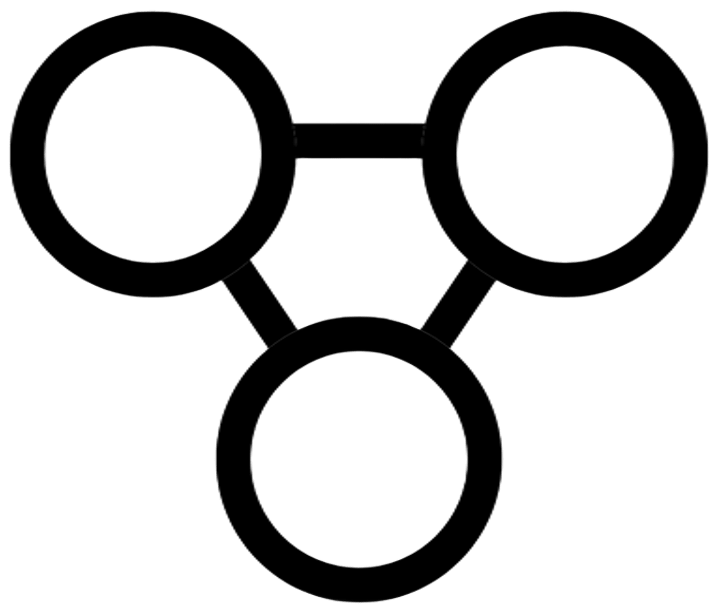
\includegraphics[width=0.46in]{bglogo2d.png}
\end{minipage}%
\begin{minipage}[c]{6.25in}
  {\Large\bfseries BO Information-Selection Formula}\par
  {\small\color{bomuted}Evidence-weighted discovery ranking and build-readiness rule}\par
\end{minipage}

\vspace{0.25em}
\hrule
\vspace{0.7em}

\textbf{1. Rank each unresolved information requirement}

\begin{equation*}
\boxed{
R(r)=P(r)+30\,\mathbf{1}\!\left[C_r\cap A\neq\varnothing\right]+10\lvert E_r\rvert
}
\end{equation*}

\begin{equation*}
P(r)=
\begin{cases}
300, & \text{if }r\text{ is critical},\\
200, & \text{if }r\text{ is high priority},\\
100, & \text{if }r\text{ is medium priority}.
\end{cases}
\end{equation*}

\begin{tabular}{>{\bfseries}p{0.85in} p{5.85in}}
$r$ & An unresolved operating-information requirement.\\
$C_r$ & Capabilities whose inclusion or design depends on requirement $r$.\\
$A$ & Capabilities currently active in the proposed Command Center.\\
$E_r$ & Matching evidence already found in the conversation.\\
$\mathbf{1}[\cdot]$ & Indicator function: $1$ when the condition is true, otherwise $0$.\\
\end{tabular}

\textbf{2. Select the highest-value unresolved requirement}

\begin{equation*}
\boxed{
r^{*}=\operatorname*{arg\,max}_{r\in U}R(r)
}
\end{equation*}

where $U$ is the set of unresolved requirements. BO converts $r^{*}$ into one short natural-language question.

\textbf{3. Stop discovery only when the build is ready}

\begin{equation*}
\boxed{
\operatorname{Ready}=
\left(\lvert U_{\mathrm{critical}}\rvert=0\right)
\land
\left(
\frac{\displaystyle\sum_{d\in D_{\mathrm{resolved}}}w_d}
     {\displaystyle\sum_{d\in D}w_d}
\geq 0.35
\right)
}
\end{equation*}

The dimension weights are

\begin{equation*}
\begin{aligned}
&w_{\mathrm{offering}}=5,\quad
w_{\mathrm{revenue}}=4.5,\quad
w_{\mathrm{delivery}}=4,\quad
w_{\mathrm{customer}}=3.5,\\
&w_{\mathrm{workforce}}=3,\quad
w_{\mathrm{supply}}=2.5,\quad
w_{\mathrm{control}}=2.
\end{aligned}
\end{equation*}

\vfill
{\footnotesize\color{bomuted}
Implementation references: \texttt{src/engine/knowledgeEngine.ts},
\texttt{src/engine/businessResearch.ts}, and
\texttt{src/engine/discoveryModel.ts}.}

\end{document}
